\documentclass[20pt,landscape]{foils}
\usepackage{mbtslides}
\usepackage[english]{babel}
\usepackage{graphicx}
\usepackage{marvosym}
\usepackage{amssymb}  % provides \gtrsim
\usepackage{ellipse}
\usepackage{fancyvrb}
\usepackage{ulem}  % provides \sout
\usepackage[cm]{sfmath}

\newif\ifrubric
% \rubrictrue

% This is supposed to make underscores cut'n'pastable
% Not sure what the lmodern package does or whether it's needed for this.
% But it's not working (though apparently it did in nam2023)
% \usepackage[T1]{fontenc}
% \usepackage{lmodern}
% \usepackage{textcomp}
% \DeclareTextSymbolDefault{\textunderscore}{T1}

\setlength{\unitlength}{1cm}


\newcommand{\bhref}[2]{\href{#1}{{\color{blue}#2}}}
\newcommand{\burl}[1]{{\color{blue}\url{#1}}}
\newcommand{\rfc}[1]{\bhref{https://www.rfc-editor.org/rfc/rfc#1}
                           {RFC\,#1}}

\newcommand{\buttimg}[1]
           {\mbox{\vtop{\vskip-2ex\hbox{\includegraphics[height=3ex]{#1}}}}}
\newcommand{\tcicon}[1]{
   \mbox{\vtop{\vskip-2.5ex\hbox{\includegraphics[height=3ex]{#1}}}}}
\newcommand{\buttitem}[1]{\item[{\makebox[0cm][r]{\tcicon{#1}}}]}
\definecolor{darkergreen}{rgb}{0,0.38,0}
\definecolor{purple}{rgb}{0.8,0,0.8}

% Fixes problem with includegraphics images screwing up colours on their
% page in the output PDF.  I have no idea *how* it fixes it mind.
\pdfpageattr {/Group << /S /Transparency /I true /CS /DeviceRGB>>}

% Oh no, this is required on my Ubuntu 22.04 (though not 20.04) installation
% to make the \ellipse commands work.
\makeatletter
\newdimen\@tempdimd
\makeatother

\begin{document}
\sf

\newcommand{\bigword}[1]{
  \vspace*{7cm}
  \begin{center}
    \color{darkblue}
    \scalebox{3}{
      \Huge\bf #1
    }
  \end{center}
  \addtocounter{page}{-1}
}

\ifrubric

\rightfooter{}
\MyLogo{}

\vspace*{3cm}
\hspace*{5cm}
\begin{minipage}{30cm}
\LARGE
\begin{enumerate}
  \item Wins
  \item Issues
  \item Ins and Outs of FITS
  \item AOB
\end{enumerate}
\end{minipage}

\newpage
\bigword{Wins?}
\newpage
\bigword{Issues?}
\newpage

\fi

\MyLogo{\color{grey}
        Mark Taylor, FITS file format,
        Bristol Astro Dev Group,
        17 January 2025}
\rightfooter{\quad{\color{grey}\thepage/\pageref*{lastPage}}}
\setcounter{page}{1}

\vspace*{1.0cm}
\begin{center}
{\color{darkblue}
\framebox{\Huge\bf
  \begin{minipage}{0cm}
  \begin{tabbing}
  Ins and Outs of FITS 
  \end{tabbing}
  \end{minipage}
}}
\\[2.0cm]
{\Large
  Mark Taylor
}
\\[2.0cm]
{\large\color{grey}
  Bristol Astro Dev Group
  \\[2ex]
  2 May 2025
}
\end{center}

\vspace*{1.5cm}
\begin{center}
  \tiny
  \color{brown}
  \input gitid
\end{center}

\slide{Outline}

\begin{list0}
  \item {\bf Flexible Image Transport System}
\end{list0}

\slide{Why am I talking about FITS?}

\begin{list1}
  \item Hattie had a problem with a FITS file that was quite easy to fix
  \begin{list2big}
    \item[] ... if you know a little bit about the format
  \end{list2big}
  \item Fergus suggested it
  \item You will have to use FITS files
  \item It's a good format for a lot of things,
        useful to know its pros and cons
\end{list1}


\slide{FITS History}

\begin{list1}
  \item Roots in the late 1970s
  \begin{list2big}
    \item Work at NRAO, Kitt Peak, Westerbork
  \end{list2big}
  \item 1981: First published proposal
        \bhref{https://ui.adsabs.harvard.edu/abs/1981A&AS...44..363W}
              {Wells, Greisen and Harten, A{\&}A {\sl 44}, p.363 (1981)}
  \begin{list2big}
    \item {\sl
           ``adoption of a unique interchange tape format to be used for
             transferring digital imagery between cooperating institutions''}
    \item Integer data only (but with provision for real scaling)
  \end{list2big}
  \item 1982: Endorsed by IAU
  \item FITS standard versions:
  \begin{list2big}
     \item[1993] v1.0 --- IEEE754 floating point values, ASCII table extension
     \item[1998] v1.2 --- IMAGE and BINTABLE extensions
     \item[2005] v2.1b --- 64-bit integers
     \item[2008] v3.0 --- WCS (celestial and spectral)
     \item[2018] v4.0 --- compression, long string keywords, WCS (time)
  \end{list2big}
\end{list1}

\slide{Pros and Cons}
\vspace*{-0.5cm}

\begin{list1}
  \item Standard, widely used, lots of software
\vspace*{-0.2cm}
  \begin{list2}
    \item Envied by other disciplines who lack standard formats
\vspace*{-0.1cm}
  \end{list2}
  \item Format definition is published, well-defined, readable
        (not defined by software)
  \item Stable.  Conservative.  Changes very slowly.
\vspace*{-0.2cm}
  \begin{list2}
    \item {\sl ``Once FITS forever FITS''}
\vspace*{-0.1cm}
  \end{list2}
  \item Data and metadata simple to read and write
\vspace*{-0.2cm}
  \begin{list2}
    \item By design --- initial implementations were in FORTRAN
\vspace*{-0.1cm}
    \item Data model very limited
\vspace*{-0.1cm}
    \item Metadata model primitive and flat, ASCII-only
\vspace*{-0.1cm}
  \end{list2}
  \item World Coordinate System metadata included
\vspace*{-0.2cm}
  \begin{list2}
    \item Fairly capable (sky, time, spectra) but inflexible
\vspace*{-0.1cm}
  \end{list2}
  \item Predictable layout of image and table data
\vspace*{-0.2cm}
  \begin{list2}
    \item Good for memory mapping and random access
\vspace*{-0.1cm}
  \end{list2}
  \item Some content restrictions
\vspace*{-0.2cm}
  \begin{list2}
    \item $\le$999 table columns (and $\le$999 image dimensions)
\vspace*{-0.1cm}
    \item Not possible to stream table data (row count required up front)
\vspace*{-0.1cm}
    \item Not optimised for parallel I/O
\vspace*{-0.1cm}
  \end{list2}
\end{list1}

\slide{Love it or hate it?}

\begin{picture}(30,0)
  \put(24,-8){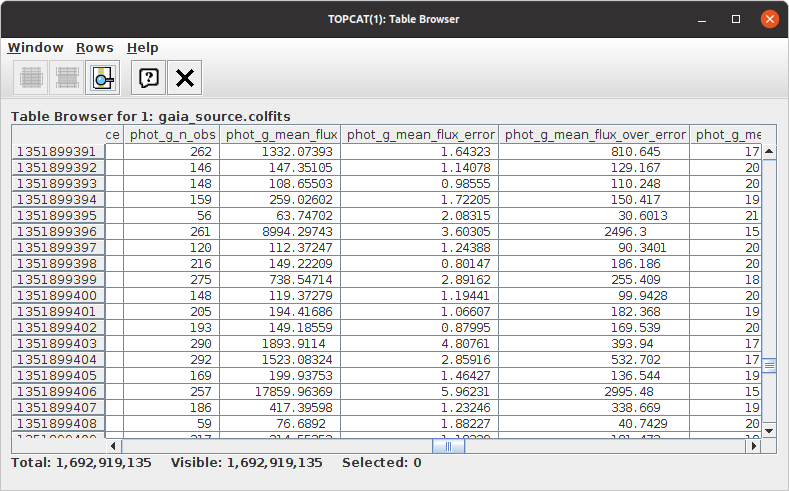
\includegraphics[scale=0.45]{JTable-gaia_source.png}}
  \put(22,-10){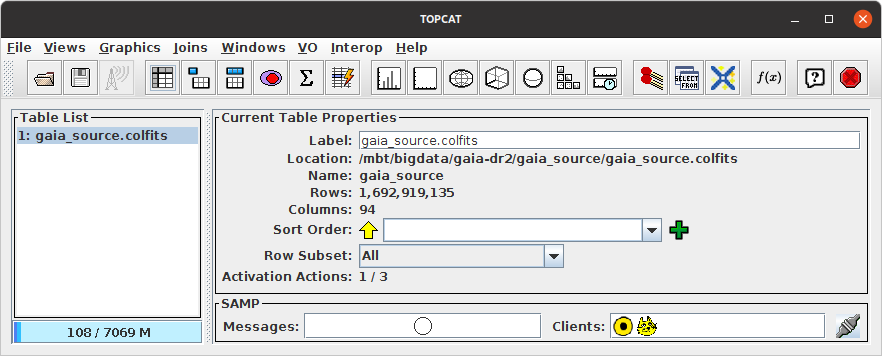
\includegraphics[scale=0.45]{topcat-gaia_source.png}}
\end{picture}
\vspace*{-1.5cm}

\begin{list1}
  \item I like it
  \begin{list2big}
    \item Great for memory-mapped data access in TOPCAT/STILTS
    \item Easy to write a performant I/O library
  \end{list2big}
  \item The Pope likes (liked) it
  \begin{list2big}
    \item In 2010 the Vatican library 
          \bhref{https://www.vaticanlibrary.va/en/the-collections/in-digitalizzation.html}
                {announced decision} \\
          to digitise 80k documents using FITS
  \end{list2big}
  \item The astronomy community is ambivalent
  \begin{list2big}
    \item There are frequent attempts to move \\
          to more modern/capable formats \\
          (HDF5, ASDF, VOTable, Parquet, ...)
    \item Papers published bemoaning FITS limitations,
          \\ e.g.\
          \bhref{https://ui.adsabs.harvard.edu/abs/2015A&C....12..133T}
                {Thomas et al., A\&C {\sl 12}, p.133 (2015)}
    \item But FITS keeps not dying
  \end{list2big}
\end{list1}

\slide{Format Overview}

\begin{picture}(30,0)
  \put(23,-15){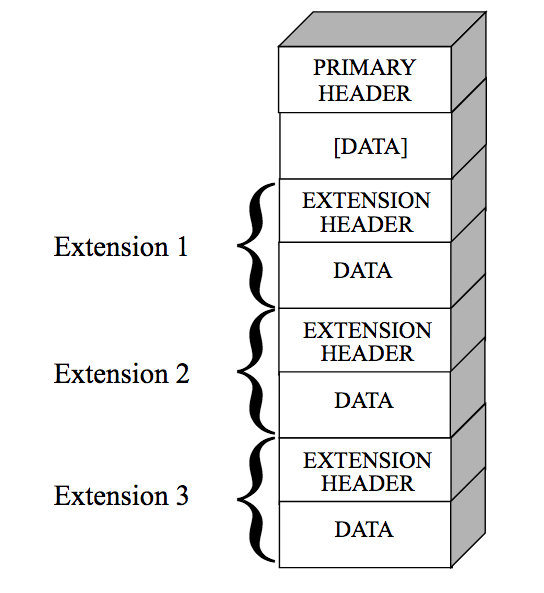
\includegraphics[height=15cm]{fig31_fitsformat.png}}
  \put(32,-16){{\small Credit: \bhref{https://hst-docs.stsci.edu/hstdhb/3-hst-file-formats/3-2-fits-file-format}{STScI}}}
\end{picture}
\vspace*{-1.5cm}

\begin{list0}
  \item Organisation of a FITS file:
  \begin{list2}
    \item Sequence of Header $+$ Data Units (HDUs)
\vspace*{-0.2cm}
    \begin{list3}
      \item Exactly one Primary HDU (PHDU)
      \begin{list4}
        \item Data (if present) must be image-like
      \end{list4}
      \item Zero or more Extension HDUs
      \begin{list4}
        \item Data (if present) may be image- or table-like
              (or, rarely, other things)
      \end{list4}
    \end{list3}
\vspace*{-0.2cm}
    \item Each HDU has a Header part and, optionally, a Data part
\vspace*{-0.2cm}
    \item Image data is an N-dimensional array of a single primitive data type
\vspace*{-0.2cm}
    \item Table data is a sequence of rows of typed columns 
\vspace*{-0.2cm}
    \begin{list3}
      \item Each column type is a primitive or N-dimensional array of primitives
    \end{list3}
\vspace*{-0.2cm}
    \item Primitive data types are big-endian 8/16/32/64-bit ints,
                                              32/64-bit IEEE754 floats
    \begin{list3}
      \item No strings as such, but you can use arrays of bytes (ASCII)
    \end{list3}
\vspace*{-0.2cm}
    \item Arrays are column-major (like FORTRAN, not like C/Python)
\vspace*{-0.2cm}
    \item File consists of 2880-byte blocks
\vspace*{-0.2cm}
    \begin{list3}
      \item Header and Data parts aligned on block boundaries, must pad to end
      \item File length is \underline{always} a multiple of 2880
            \hspace*{1em} {\color{darkred}\sl $\leftarrow$ useful fact!}
      \item[] \hspace*{1.5em}
              \begin{minipage}{25cm}
                {\sl\small\color{darkgrey}
                ``All records will have a length of 23040 bits
                  (2880 8-bit bytes, 3840 6-bit bytes).\\
                  This length is evenly divisible by both the byte and word
                  lengths of all computers \\
                  that have been sold in the commercial market
                  (i.e., 6, 8, 12, 16, 18, 24, 32, \\
                  36, 48, 60 and 64 bits)''}
              \end{minipage}
    \end{list3}
  \end{list2}
\end{list0}

\slide{Header Format}

\begin{list0}
\vspace*{-0.1cm}
  \item Header is a sequence of 80-character ``cards''
\vspace*{-0.1cm}
  \begin{list2big}
    \item Mostly {\color{brown}\tt KEY = value}
    \begin{list3}
      \item Fixed format:
            {\color{brown}\verb*|KEY      = value... / comment...|}
      \item Keyword is $\le 8$ characters,
            {\color{brown}\verb|[A-Z0-9_-]|}
      \item Value is 7-bit ASCII string, integer, float, complex or boolean
      \item Trailing spaces in keyword and string values not significant
    \end{list3}
\vspace*{-0.1cm}
    \item Some other miscellaneous card types:
\vspace*{-0.1cm}
    \begin{list3}
      \item {\color{brown}\tt COMMENT},
            {\color{brown}\tt HISTORY},
            {\color{brown}\tt CONTINUE},
            {\color{brown}\tt END},
            blank record
    \end{list3}
\vspace*{-0.1cm}
    \item Some keywords defined by FITS standard
\vspace*{-0.1cm}
    \begin{list3}
      \item Mandatory: define layout of data unit
      \begin{list4}
        \item[] {\color{brown}\tt SIMPLE},
                {\color{brown}\tt EXTENSION},
                {\color{brown}\tt BITPIX},
                {\color{brown}\tt NAXIS},
                {\color{brown}\tt PCOUNT},
                ...
      \end{list4}
      \item Reserved: useful items to describe data and metadata, incl.\ WCS
      \begin{list4}
        \item[] {\color{brown}\tt DATE},
                {\color{brown}\tt BSCALE},
                {\color{brown}\tt BUNIT},
                {\color{brown}\tt DATAMAX},
                {\color{brown}\tt TELESCOP},
                {\color{brown}\tt TTYPEn},
                {\color{brown}\tt WCSAXESa}, ...
      \end{list4}
      \item Otherwise: add any headers you want! (subject to syntax)
      \begin{list4}
        \item Write down somewhere what they mean ... or don't ...
        \item There is a
              \bhref{https://fits.gsfc.nasa.gov/fits_conventions.html}
                    {Registry of FITS conventions}
      \end{list4}
    \end{list3}
\vspace*{-0.1cm}
    \item Last record must be ``{\color{brown}\tt END}''
\vspace*{-0.1cm}
    \item Pad with spaces to end of 2880-character block
\vspace*{-0.1cm}
  \end{list2big}
\end{list0}


\slide{Tools}

\begin{list2}
  \item more
  \item vi -b
  \item FTOOLS
  \begin{list3}
    \item fverify 
    \item lots more
  \end{list3}
  \item \bhref{https://fits.gsfc.nasa.gov/fits_verify.html}{online fitsverify}
        --- limit 40Mb
\end{list2}

\slide{Summary}

\vspace{0.2cm}
\begin{center}
  {\color{darkred}\Huge\bf\sl Thanks!}
\end{center}

\label{lastPage}

\ifrubric

\newcommand{\aobSlide}[1]{
\newpage
\rightfooter{}
\MyLogo{}
\begin{picture}(30,0)
  #1
\end{picture}
\bigword{AOB?}
}
\aobSlide{}

\fi

\end{document}

